\documentclass[twoside]{book}

% Packages required by doxygen
\usepackage{fixltx2e}
\usepackage{calc}
\usepackage{doxygen}
\usepackage[export]{adjustbox} % also loads graphicx
\usepackage{graphicx}
\usepackage[utf8]{inputenc}
\usepackage{makeidx}
\usepackage{multicol}
\usepackage{multirow}
\PassOptionsToPackage{warn}{textcomp}
\usepackage{textcomp}
\usepackage[nointegrals]{wasysym}
\usepackage[table]{xcolor}

% Font selection
\usepackage[T1]{fontenc}
\usepackage[scaled=.90]{helvet}
\usepackage{courier}
\usepackage{amssymb}
\usepackage{sectsty}
\renewcommand{\familydefault}{\sfdefault}
\allsectionsfont{%
  \fontseries{bc}\selectfont%
  \color{darkgray}%
}
\renewcommand{\DoxyLabelFont}{%
  \fontseries{bc}\selectfont%
  \color{darkgray}%
}
\newcommand{\+}{\discretionary{\mbox{\scriptsize$\hookleftarrow$}}{}{}}

% Page & text layout
\usepackage{geometry}
\geometry{%
  a4paper,%
  top=2.5cm,%
  bottom=2.5cm,%
  left=2.5cm,%
  right=2.5cm%
}
\tolerance=750
\hfuzz=15pt
\hbadness=750
\setlength{\emergencystretch}{15pt}
\setlength{\parindent}{0cm}
\setlength{\parskip}{3ex plus 2ex minus 2ex}
\makeatletter
\renewcommand{\paragraph}{%
  \@startsection{paragraph}{4}{0ex}{-1.0ex}{1.0ex}{%
    \normalfont\normalsize\bfseries\SS@parafont%
  }%
}
\renewcommand{\subparagraph}{%
  \@startsection{subparagraph}{5}{0ex}{-1.0ex}{1.0ex}{%
    \normalfont\normalsize\bfseries\SS@subparafont%
  }%
}
\makeatother

% Headers & footers
\usepackage{fancyhdr}
\pagestyle{fancyplain}
\fancyhead[LE]{\fancyplain{}{\bfseries\thepage}}
\fancyhead[CE]{\fancyplain{}{}}
\fancyhead[RE]{\fancyplain{}{\bfseries\leftmark}}
\fancyhead[LO]{\fancyplain{}{\bfseries\rightmark}}
\fancyhead[CO]{\fancyplain{}{}}
\fancyhead[RO]{\fancyplain{}{\bfseries\thepage}}
\fancyfoot[LE]{\fancyplain{}{}}
\fancyfoot[CE]{\fancyplain{}{}}
\fancyfoot[RE]{\fancyplain{}{\bfseries\scriptsize Generated by Doxygen }}
\fancyfoot[LO]{\fancyplain{}{\bfseries\scriptsize Generated by Doxygen }}
\fancyfoot[CO]{\fancyplain{}{}}
\fancyfoot[RO]{\fancyplain{}{}}
\renewcommand{\footrulewidth}{0.4pt}
\renewcommand{\chaptermark}[1]{%
  \markboth{#1}{}%
}
\renewcommand{\sectionmark}[1]{%
  \markright{\thesection\ #1}%
}

% Indices & bibliography
\usepackage{natbib}
\usepackage[titles]{tocloft}
\setcounter{tocdepth}{3}
\setcounter{secnumdepth}{5}
\makeindex

% Hyperlinks (required, but should be loaded last)
\usepackage{ifpdf}
\ifpdf
  \usepackage[pdftex,pagebackref=true]{hyperref}
\else
  \usepackage[ps2pdf,pagebackref=true]{hyperref}
\fi
\hypersetup{%
  colorlinks=true,%
  linkcolor=blue,%
  citecolor=blue,%
  unicode%
}

% Custom commands
\newcommand{\clearemptydoublepage}{%
  \newpage{\pagestyle{empty}\cleardoublepage}%
}

\usepackage{caption}
\captionsetup{labelsep=space,justification=centering,font={bf},singlelinecheck=off,skip=4pt,position=top}

%===== C O N T E N T S =====

\begin{document}

% Titlepage & ToC
\hypersetup{pageanchor=false,
             bookmarksnumbered=true,
             pdfencoding=unicode
            }
\pagenumbering{roman}
\begin{titlepage}
\vspace*{7cm}
\begin{center}%
{\Large Resistance calculation library \\[1ex]\large 1 }\\
\vspace*{1cm}
{\large Generated by Doxygen 1.8.11}\\
\end{center}
\end{titlepage}
\clearemptydoublepage
\tableofcontents
\clearemptydoublepage
\pagenumbering{arabic}
\hypersetup{pageanchor=true}

%--- Begin generated contents ---
\chapter{Readme}
\label{md_Readme}
\hypertarget{md_Readme}{}
\input{md_Readme}
\chapter{File Index}
\section{File List}
Here is a list of all documented files with brief descriptions\+:\begin{DoxyCompactList}
\item\contentsline{section}{\hyperlink{libresistance_8c}{libresistance.\+c} }{\pageref{libresistance_8c}}{}
\item\contentsline{section}{\hyperlink{libresistance_8h}{libresistance.\+h} }{\pageref{libresistance_8h}}{}
\item\contentsline{section}{\hyperlink{test__main_8c}{test\+\_\+main.\+c} }{\pageref{test__main_8c}}{}
\end{DoxyCompactList}

\chapter{File Documentation}
\hypertarget{libresistance_8c}{}\section{libresistance.\+c File Reference}
\label{libresistance_8c}\index{libresistance.\+c@{libresistance.\+c}}
{\ttfamily \#include \char`\"{}stdio.\+h\char`\"{}}\\*
{\ttfamily \#include \char`\"{}libresistance.\+h\char`\"{}}\\*
Include dependency graph for libresistance.\+c\+:\nopagebreak
\begin{figure}[H]
\begin{center}
\leavevmode
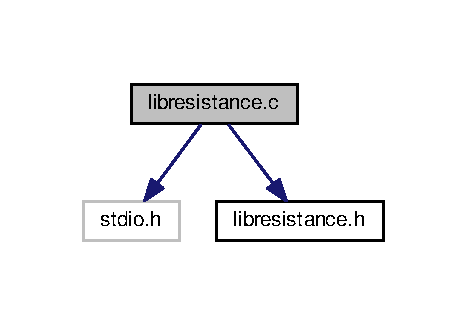
\includegraphics[width=224pt]{libresistance_8c__incl}
\end{center}
\end{figure}
\subsection*{Functions}
\begin{DoxyCompactItemize}
\item 
unsigned \hyperlink{libresistance_8c_a9a6b027f3262084b6d01e4daa6f7da3a}{has\+Invalid\+Arguments} (int count, char conn, float $\ast$array)
\begin{DoxyCompactList}\small\item\em Checks if any of the arguments are incorrect. \end{DoxyCompactList}\item 
float \hyperlink{libresistance_8c_a339b5f0f336eb492e36f9d6467678440}{calc\+\_\+resistance} (int count, char conn, float $\ast$array)
\begin{DoxyCompactList}\small\item\em Calculate the resistance for either parallell or serial connections. \end{DoxyCompactList}\end{DoxyCompactItemize}


\subsection{Function Documentation}
\index{libresistance.\+c@{libresistance.\+c}!calc\+\_\+resistance@{calc\+\_\+resistance}}
\index{calc\+\_\+resistance@{calc\+\_\+resistance}!libresistance.\+c@{libresistance.\+c}}
\subsubsection[{\texorpdfstring{calc\+\_\+resistance(int count, char conn, float $\ast$array)}{calc_resistance(int count, char conn, float *array)}}]{\setlength{\rightskip}{0pt plus 5cm}float calc\+\_\+resistance (
\begin{DoxyParamCaption}
\item[{int}]{count, }
\item[{char}]{conn, }
\item[{float $\ast$}]{array}
\end{DoxyParamCaption}
)}\hypertarget{libresistance_8c_a339b5f0f336eb492e36f9d6467678440}{}\label{libresistance_8c_a339b5f0f336eb492e36f9d6467678440}


Calculate the resistance for either parallell or serial connections. 

Calculates the resistance values for either a series of components that are connected in parallell or serial. 
\begin{DoxyParams}{Parameters}
{\em count} & The number of components \\
\hline
{\em conn} & The type of connection, can be either P(\+Parallell) or S(\+Serial) \\
\hline
{\em $\ast$array} & The resistance values of the components \\
\hline
\end{DoxyParams}
\begin{DoxyReturn}{Returns}
The summarized resistance value. If any of the input arguments are incorrect, -\/1 will be returned. 
\end{DoxyReturn}


Here is the call graph for this function\+:\nopagebreak
\begin{figure}[H]
\begin{center}
\leavevmode
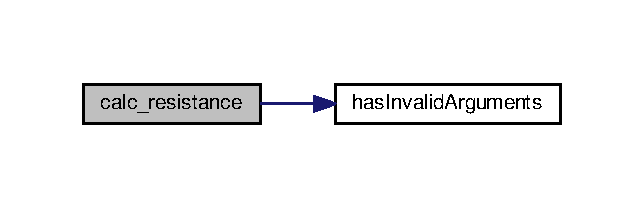
\includegraphics[width=309pt]{libresistance_8c_a339b5f0f336eb492e36f9d6467678440_cgraph}
\end{center}
\end{figure}




Here is the caller graph for this function\+:\nopagebreak
\begin{figure}[H]
\begin{center}
\leavevmode
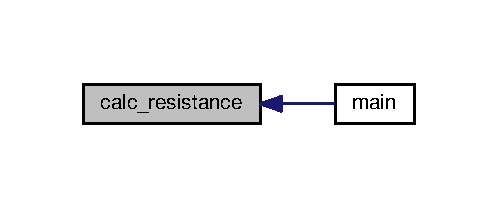
\includegraphics[width=239pt]{libresistance_8c_a339b5f0f336eb492e36f9d6467678440_icgraph}
\end{center}
\end{figure}


\index{libresistance.\+c@{libresistance.\+c}!has\+Invalid\+Arguments@{has\+Invalid\+Arguments}}
\index{has\+Invalid\+Arguments@{has\+Invalid\+Arguments}!libresistance.\+c@{libresistance.\+c}}
\subsubsection[{\texorpdfstring{has\+Invalid\+Arguments(int count, char conn, float $\ast$array)}{hasInvalidArguments(int count, char conn, float *array)}}]{\setlength{\rightskip}{0pt plus 5cm}unsigned has\+Invalid\+Arguments (
\begin{DoxyParamCaption}
\item[{int}]{count, }
\item[{char}]{conn, }
\item[{float $\ast$}]{array}
\end{DoxyParamCaption}
)}\hypertarget{libresistance_8c_a9a6b027f3262084b6d01e4daa6f7da3a}{}\label{libresistance_8c_a9a6b027f3262084b6d01e4daa6f7da3a}


Checks if any of the arguments are incorrect. 

Checks if any of the arguments are incorrect. It checks\+: conn is P or S count is larger than 0 array is not an empty array 
\begin{DoxyParams}{Parameters}
{\em count} & The number of components \\
\hline
{\em conn} & The type of connection, can be either P(\+Parallell) or S(\+Serial) \\
\hline
{\em $\ast$array} & The resistance values of the components \\
\hline
\end{DoxyParams}
\begin{DoxyReturn}{Returns}
Returns -\/1 if any of the arguments is incorrect, otherwise 0. 
\end{DoxyReturn}


Here is the caller graph for this function\+:\nopagebreak
\begin{figure}[H]
\begin{center}
\leavevmode
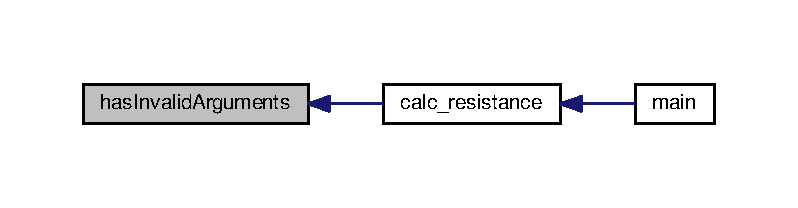
\includegraphics[width=350pt]{libresistance_8c_a9a6b027f3262084b6d01e4daa6f7da3a_icgraph}
\end{center}
\end{figure}



\hypertarget{libresistance_8h}{}\section{libresistance.\+h File Reference}
\label{libresistance_8h}\index{libresistance.\+h@{libresistance.\+h}}
This graph shows which files directly or indirectly include this file\+:\nopagebreak
\begin{figure}[H]
\begin{center}
\leavevmode
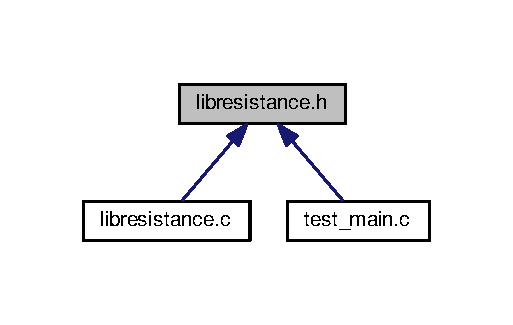
\includegraphics[width=246pt]{libresistance_8h__dep__incl}
\end{center}
\end{figure}
\subsection*{Functions}
\begin{DoxyCompactItemize}
\item 
float \hyperlink{libresistance_8h_a339b5f0f336eb492e36f9d6467678440}{calc\+\_\+resistance} (int count, char conn, float $\ast$array)
\begin{DoxyCompactList}\small\item\em Calculate the resistance for either parallell or serial connections. \end{DoxyCompactList}\end{DoxyCompactItemize}


\subsection{Function Documentation}
\index{libresistance.\+h@{libresistance.\+h}!calc\+\_\+resistance@{calc\+\_\+resistance}}
\index{calc\+\_\+resistance@{calc\+\_\+resistance}!libresistance.\+h@{libresistance.\+h}}
\subsubsection[{\texorpdfstring{calc\+\_\+resistance(int count, char conn, float $\ast$array)}{calc_resistance(int count, char conn, float *array)}}]{\setlength{\rightskip}{0pt plus 5cm}float calc\+\_\+resistance (
\begin{DoxyParamCaption}
\item[{int}]{count, }
\item[{char}]{conn, }
\item[{float $\ast$}]{array}
\end{DoxyParamCaption}
)}\hypertarget{libresistance_8h_a339b5f0f336eb492e36f9d6467678440}{}\label{libresistance_8h_a339b5f0f336eb492e36f9d6467678440}


Calculate the resistance for either parallell or serial connections. 

Calculates the resistance values for either a series of components that are connected in parallell or serial. 
\begin{DoxyParams}{Parameters}
{\em count} & The number of components \\
\hline
{\em conn} & The type of connection, can be either P(\+Parallell) or S(\+Serial) \\
\hline
{\em $\ast$array} & The resistance values of the components \\
\hline
\end{DoxyParams}
\begin{DoxyReturn}{Returns}
The summarized resistance value. If any of the input arguments are incorrect, -\/1 will be returned. 
\end{DoxyReturn}


Here is the call graph for this function\+:\nopagebreak
\begin{figure}[H]
\begin{center}
\leavevmode
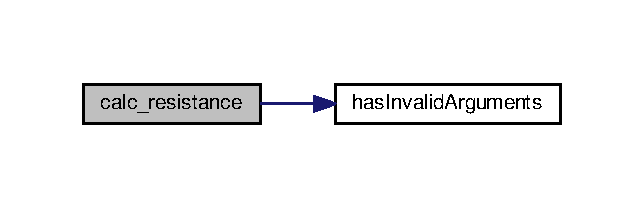
\includegraphics[width=309pt]{libresistance_8h_a339b5f0f336eb492e36f9d6467678440_cgraph}
\end{center}
\end{figure}




Here is the caller graph for this function\+:\nopagebreak
\begin{figure}[H]
\begin{center}
\leavevmode
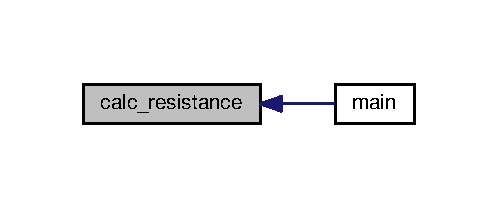
\includegraphics[width=239pt]{libresistance_8h_a339b5f0f336eb492e36f9d6467678440_icgraph}
\end{center}
\end{figure}



\hypertarget{test__main_8c}{}\section{test\+\_\+main.\+c File Reference}
\label{test__main_8c}\index{test\+\_\+main.\+c@{test\+\_\+main.\+c}}
{\ttfamily \#include $<$stdio.\+h$>$}\\*
{\ttfamily \#include $<$stdlib.\+h$>$}\\*
{\ttfamily \#include $<$stdarg.\+h$>$}\\*
{\ttfamily \#include $<$assert.\+h$>$}\\*
{\ttfamily \#include $<$string.\+h$>$}\\*
{\ttfamily \#include \char`\"{}libresistance.\+h\char`\"{}}\\*
Include dependency graph for test\+\_\+main.\+c\+:\nopagebreak
\begin{figure}[H]
\begin{center}
\leavevmode
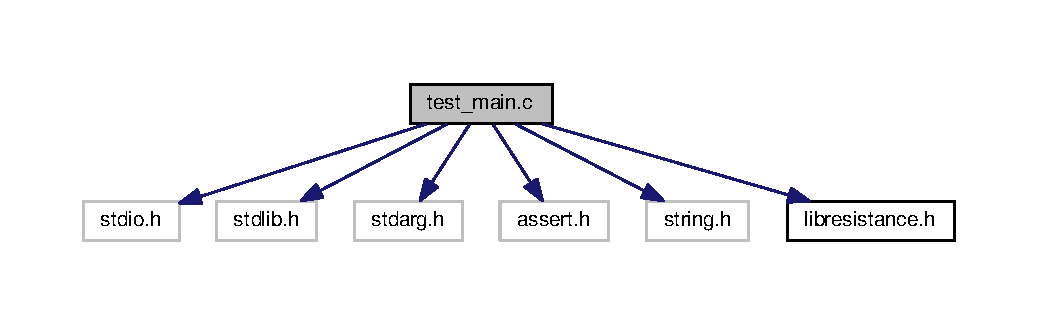
\includegraphics[width=350pt]{test__main_8c__incl}
\end{center}
\end{figure}
\subsection*{Macros}
\begin{DoxyCompactItemize}
\item 
\#define \hyperlink{test__main_8c_a34995b955465f6bbb37c359173d50477}{A\+N\+S\+I\+\_\+\+C\+O\+L\+O\+R\+\_\+\+R\+ED}~\char`\"{}\textbackslash{}x1b\mbox{[}31m\char`\"{}\hypertarget{test__main_8c_a34995b955465f6bbb37c359173d50477}{}\label{test__main_8c_a34995b955465f6bbb37c359173d50477}

\begin{DoxyCompactList}\small\item\em Defines the red colour. \end{DoxyCompactList}\item 
\#define \hyperlink{test__main_8c_a966c72d8d733c7734c6c784753d894c7}{A\+N\+S\+I\+\_\+\+C\+O\+L\+O\+R\+\_\+\+G\+R\+E\+EN}~\char`\"{}\textbackslash{}x1b\mbox{[}32m\char`\"{}\hypertarget{test__main_8c_a966c72d8d733c7734c6c784753d894c7}{}\label{test__main_8c_a966c72d8d733c7734c6c784753d894c7}

\begin{DoxyCompactList}\small\item\em Defines the green colour. \end{DoxyCompactList}\end{DoxyCompactItemize}
\subsection*{Enumerations}
\begin{DoxyCompactItemize}
\item 
enum \hyperlink{test__main_8c_a7c6368b321bd9acd0149b030bb8275ed}{boolean} \{ \hyperlink{test__main_8c_a7c6368b321bd9acd0149b030bb8275edaa1e095cc966dbecf6a0d8aad75348d1a}{F\+A\+L\+SE} = 0, 
\hyperlink{test__main_8c_a7c6368b321bd9acd0149b030bb8275edaa82764c3079aea4e60c80e45befbb839}{T\+R\+UE}
 \}\begin{DoxyCompactList}\small\item\em To avoid having to use 1 and 0, there is an enum definition that mimics true and false. \end{DoxyCompactList}
\end{DoxyCompactItemize}
\subsection*{Functions}
\begin{DoxyCompactItemize}
\item 
void \hyperlink{test__main_8c_a3cce6cf3c9672ca1aa12539a4d0a2ffd}{print\+Test\+Text} (char $\ast$test\+Name, char $\ast$text, char $\ast$colour, va\+\_\+list args)
\begin{DoxyCompactList}\small\item\em Prints a text with a given colour and a list of arguments. \end{DoxyCompactList}\item 
void \hyperlink{test__main_8c_a66f18f87f6441f456b913891011961f2}{print\+Failed\+Test\+Text} (char $\ast$test\+Name, char $\ast$text,...)
\begin{DoxyCompactList}\small\item\em Prints failing test messages. \end{DoxyCompactList}\item 
void \hyperlink{test__main_8c_a88f8707e23480970b8ab040b43e6de1f}{print\+Success\+Test\+Text} (char $\ast$test\+Name, char $\ast$text,...)
\begin{DoxyCompactList}\small\item\em Prints successful test messages. \end{DoxyCompactList}\item 
unsigned \hyperlink{test__main_8c_abc90911659e645bbb1d2de847e25b493}{assert\+Is\+The\+Same} (char $\ast$test\+Name, float expected, float given)
\begin{DoxyCompactList}\small\item\em Test method that is used to check if two floats are the same. \end{DoxyCompactList}\item 
unsigned \hyperlink{test__main_8c_aa3162138d18e941d0b61ee83136e9d9c}{assert\+Is\+Not\+The\+Same} (char $\ast$test\+Name, float expected, float given)
\begin{DoxyCompactList}\small\item\em Test method that is used to check if two floats are not the same. \end{DoxyCompactList}\item 
int \hyperlink{test__main_8c_ae66f6b31b5ad750f1fe042a706a4e3d4}{main} ()
\begin{DoxyCompactList}\small\item\em Runs all the tests. \end{DoxyCompactList}\end{DoxyCompactItemize}


\subsection{Enumeration Type Documentation}
\index{test\+\_\+main.\+c@{test\+\_\+main.\+c}!boolean@{boolean}}
\index{boolean@{boolean}!test\+\_\+main.\+c@{test\+\_\+main.\+c}}
\subsubsection[{\texorpdfstring{boolean}{boolean}}]{\setlength{\rightskip}{0pt plus 5cm}enum {\bf boolean}}\hypertarget{test__main_8c_a7c6368b321bd9acd0149b030bb8275ed}{}\label{test__main_8c_a7c6368b321bd9acd0149b030bb8275ed}


To avoid having to use 1 and 0, there is an enum definition that mimics true and false. 

\begin{Desc}
\item[Enumerator]\par
\begin{description}
\index{F\+A\+L\+SE@{F\+A\+L\+SE}!test\+\_\+main.\+c@{test\+\_\+main.\+c}}\index{test\+\_\+main.\+c@{test\+\_\+main.\+c}!F\+A\+L\+SE@{F\+A\+L\+SE}}\item[{\em 
F\+A\+L\+SE\hypertarget{test__main_8c_a7c6368b321bd9acd0149b030bb8275edaa1e095cc966dbecf6a0d8aad75348d1a}{}\label{test__main_8c_a7c6368b321bd9acd0149b030bb8275edaa1e095cc966dbecf6a0d8aad75348d1a}
}]The same as 0. \index{T\+R\+UE@{T\+R\+UE}!test\+\_\+main.\+c@{test\+\_\+main.\+c}}\index{test\+\_\+main.\+c@{test\+\_\+main.\+c}!T\+R\+UE@{T\+R\+UE}}\item[{\em 
T\+R\+UE\hypertarget{test__main_8c_a7c6368b321bd9acd0149b030bb8275edaa82764c3079aea4e60c80e45befbb839}{}\label{test__main_8c_a7c6368b321bd9acd0149b030bb8275edaa82764c3079aea4e60c80e45befbb839}
}]The same as 1. \end{description}
\end{Desc}


\subsection{Function Documentation}
\index{test\+\_\+main.\+c@{test\+\_\+main.\+c}!assert\+Is\+Not\+The\+Same@{assert\+Is\+Not\+The\+Same}}
\index{assert\+Is\+Not\+The\+Same@{assert\+Is\+Not\+The\+Same}!test\+\_\+main.\+c@{test\+\_\+main.\+c}}
\subsubsection[{\texorpdfstring{assert\+Is\+Not\+The\+Same(char $\ast$test\+Name, float expected, float given)}{assertIsNotTheSame(char *testName, float expected, float given)}}]{\setlength{\rightskip}{0pt plus 5cm}unsigned assert\+Is\+Not\+The\+Same (
\begin{DoxyParamCaption}
\item[{char $\ast$}]{test\+Name, }
\item[{float}]{expected, }
\item[{float}]{given}
\end{DoxyParamCaption}
)}\hypertarget{test__main_8c_aa3162138d18e941d0b61ee83136e9d9c}{}\label{test__main_8c_aa3162138d18e941d0b61ee83136e9d9c}


Test method that is used to check if two floats are not the same. 

Compare two float values and returns 1 if it\textquotesingle{}s not the same and 0 if it is. It allso makes an assert(expected != given). 
\begin{DoxyParams}{Parameters}
{\em test\+Name} & The name of the test \\
\hline
{\em expected} & The value to expect \\
\hline
{\em given} & The value returned by the test \\
\hline
\end{DoxyParams}
\begin{DoxyReturn}{Returns}
Returns 1(T\+R\+UE) if the test is ok and 0(F\+A\+L\+SE) if it\textquotesingle{}s not 
\end{DoxyReturn}


Here is the call graph for this function\+:\nopagebreak
\begin{figure}[H]
\begin{center}
\leavevmode
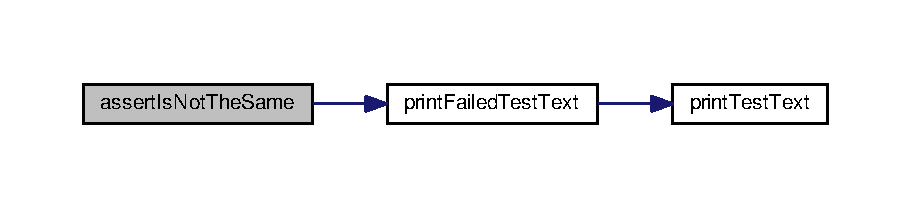
\includegraphics[width=350pt]{test__main_8c_aa3162138d18e941d0b61ee83136e9d9c_cgraph}
\end{center}
\end{figure}




Here is the caller graph for this function\+:\nopagebreak
\begin{figure}[H]
\begin{center}
\leavevmode
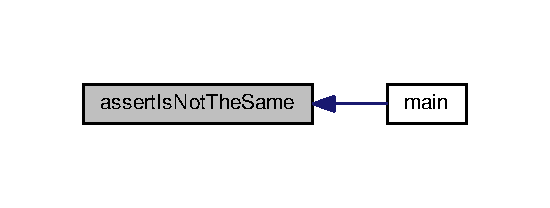
\includegraphics[width=264pt]{test__main_8c_aa3162138d18e941d0b61ee83136e9d9c_icgraph}
\end{center}
\end{figure}


\index{test\+\_\+main.\+c@{test\+\_\+main.\+c}!assert\+Is\+The\+Same@{assert\+Is\+The\+Same}}
\index{assert\+Is\+The\+Same@{assert\+Is\+The\+Same}!test\+\_\+main.\+c@{test\+\_\+main.\+c}}
\subsubsection[{\texorpdfstring{assert\+Is\+The\+Same(char $\ast$test\+Name, float expected, float given)}{assertIsTheSame(char *testName, float expected, float given)}}]{\setlength{\rightskip}{0pt plus 5cm}unsigned assert\+Is\+The\+Same (
\begin{DoxyParamCaption}
\item[{char $\ast$}]{test\+Name, }
\item[{float}]{expected, }
\item[{float}]{given}
\end{DoxyParamCaption}
)}\hypertarget{test__main_8c_abc90911659e645bbb1d2de847e25b493}{}\label{test__main_8c_abc90911659e645bbb1d2de847e25b493}


Test method that is used to check if two floats are the same. 

Compare two float values and returns 1 if it\textquotesingle{}s the same and 0 if it\textquotesingle{}s not. It allso makes an assert(expected == given). 
\begin{DoxyParams}{Parameters}
{\em test\+Name} & The name of the test \\
\hline
{\em expected} & The value to expect \\
\hline
{\em given} & The value returned by the test \\
\hline
\end{DoxyParams}
\begin{DoxyReturn}{Returns}
Returns 1(T\+R\+UE) if the test is ok and 0(F\+A\+L\+SE) if it\textquotesingle{}s not 
\end{DoxyReturn}


Here is the call graph for this function\+:\nopagebreak
\begin{figure}[H]
\begin{center}
\leavevmode
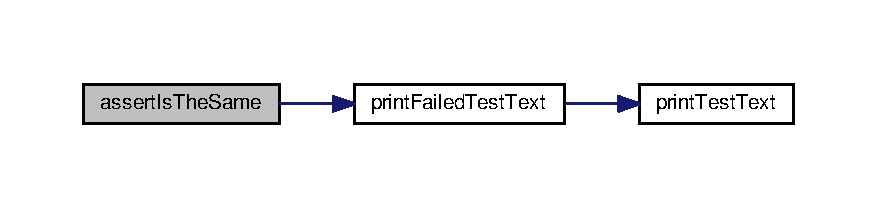
\includegraphics[width=350pt]{test__main_8c_abc90911659e645bbb1d2de847e25b493_cgraph}
\end{center}
\end{figure}




Here is the caller graph for this function\+:\nopagebreak
\begin{figure}[H]
\begin{center}
\leavevmode
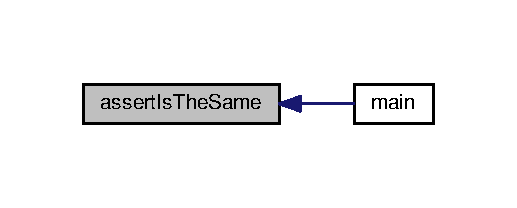
\includegraphics[width=248pt]{test__main_8c_abc90911659e645bbb1d2de847e25b493_icgraph}
\end{center}
\end{figure}


\index{test\+\_\+main.\+c@{test\+\_\+main.\+c}!main@{main}}
\index{main@{main}!test\+\_\+main.\+c@{test\+\_\+main.\+c}}
\subsubsection[{\texorpdfstring{main()}{main()}}]{\setlength{\rightskip}{0pt plus 5cm}int main (
\begin{DoxyParamCaption}
{}
\end{DoxyParamCaption}
)}\hypertarget{test__main_8c_ae66f6b31b5ad750f1fe042a706a4e3d4}{}\label{test__main_8c_ae66f6b31b5ad750f1fe042a706a4e3d4}


Runs all the tests. 

Runs all the tests and returns 0 if it\textquotesingle{}s ok and 1 if it\textquotesingle{}s not \begin{DoxyReturn}{Returns}
Returns 0 if it\textquotesingle{}s ok and 1 if it\textquotesingle{}s not ok. 
\end{DoxyReturn}


Here is the call graph for this function\+:\nopagebreak
\begin{figure}[H]
\begin{center}
\leavevmode
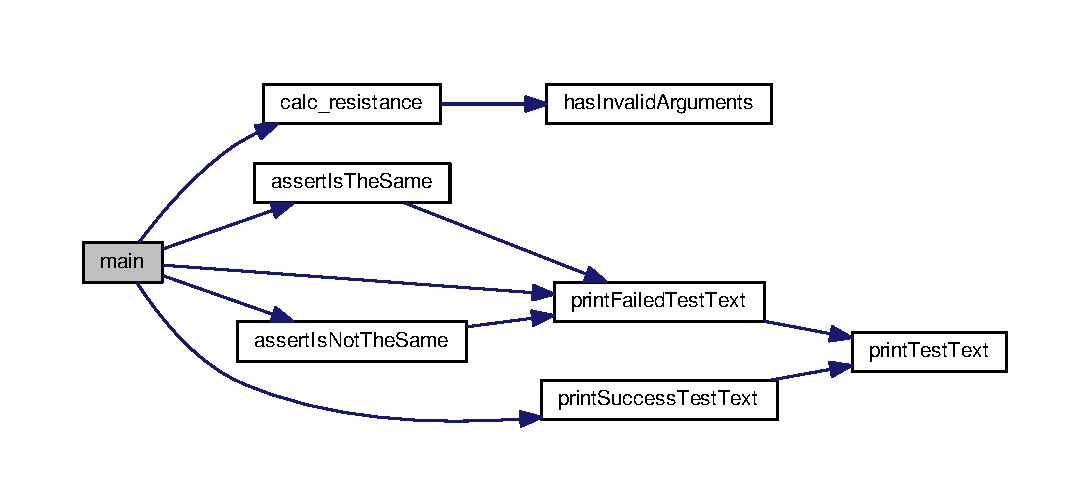
\includegraphics[width=350pt]{test__main_8c_ae66f6b31b5ad750f1fe042a706a4e3d4_cgraph}
\end{center}
\end{figure}


\index{test\+\_\+main.\+c@{test\+\_\+main.\+c}!print\+Failed\+Test\+Text@{print\+Failed\+Test\+Text}}
\index{print\+Failed\+Test\+Text@{print\+Failed\+Test\+Text}!test\+\_\+main.\+c@{test\+\_\+main.\+c}}
\subsubsection[{\texorpdfstring{print\+Failed\+Test\+Text(char $\ast$test\+Name, char $\ast$text,...)}{printFailedTestText(char *testName, char *text,...)}}]{\setlength{\rightskip}{0pt plus 5cm}void print\+Failed\+Test\+Text (
\begin{DoxyParamCaption}
\item[{char $\ast$}]{test\+Name, }
\item[{char $\ast$}]{text, }
\item[{}]{...}
\end{DoxyParamCaption}
)}\hypertarget{test__main_8c_a66f18f87f6441f456b913891011961f2}{}\label{test__main_8c_a66f18f87f6441f456b913891011961f2}


Prints failing test messages. 

Calls print\+Test\+Text function with red text as pre defined and provide the parameters sent in 
\begin{DoxyParams}{Parameters}
{\em test\+Name} & The name of the test \\
\hline
{\em text} & The text message to print out \\
\hline
\end{DoxyParams}
\begin{DoxyReturn}{Returns}
void 
\end{DoxyReturn}


Here is the call graph for this function\+:\nopagebreak
\begin{figure}[H]
\begin{center}
\leavevmode
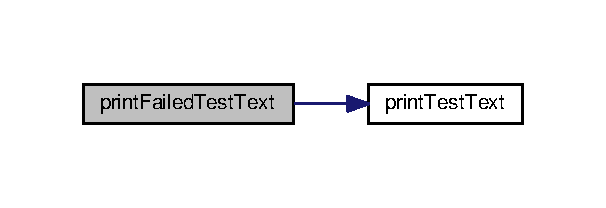
\includegraphics[width=291pt]{test__main_8c_a66f18f87f6441f456b913891011961f2_cgraph}
\end{center}
\end{figure}




Here is the caller graph for this function\+:\nopagebreak
\begin{figure}[H]
\begin{center}
\leavevmode
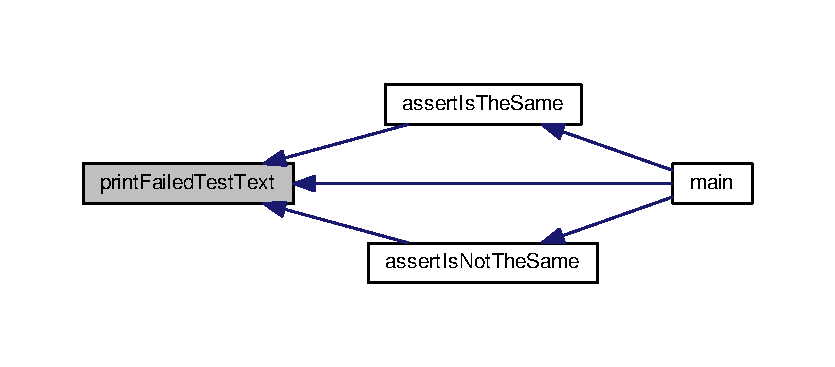
\includegraphics[width=350pt]{test__main_8c_a66f18f87f6441f456b913891011961f2_icgraph}
\end{center}
\end{figure}


\index{test\+\_\+main.\+c@{test\+\_\+main.\+c}!print\+Success\+Test\+Text@{print\+Success\+Test\+Text}}
\index{print\+Success\+Test\+Text@{print\+Success\+Test\+Text}!test\+\_\+main.\+c@{test\+\_\+main.\+c}}
\subsubsection[{\texorpdfstring{print\+Success\+Test\+Text(char $\ast$test\+Name, char $\ast$text,...)}{printSuccessTestText(char *testName, char *text,...)}}]{\setlength{\rightskip}{0pt plus 5cm}void print\+Success\+Test\+Text (
\begin{DoxyParamCaption}
\item[{char $\ast$}]{test\+Name, }
\item[{char $\ast$}]{text, }
\item[{}]{...}
\end{DoxyParamCaption}
)}\hypertarget{test__main_8c_a88f8707e23480970b8ab040b43e6de1f}{}\label{test__main_8c_a88f8707e23480970b8ab040b43e6de1f}


Prints successful test messages. 

Calls print\+Test\+Text function with green text as pre defined and provide the parameters sent in 
\begin{DoxyParams}{Parameters}
{\em test\+Name} & The name of the test \\
\hline
{\em text} & The text message to print out \\
\hline
\end{DoxyParams}
\begin{DoxyReturn}{Returns}
void 
\end{DoxyReturn}


Here is the call graph for this function\+:\nopagebreak
\begin{figure}[H]
\begin{center}
\leavevmode
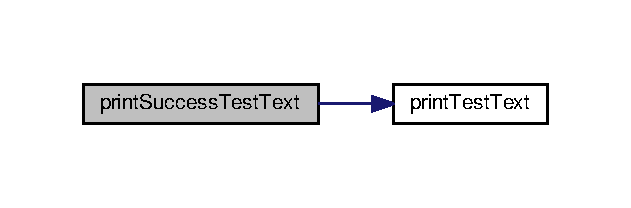
\includegraphics[width=303pt]{test__main_8c_a88f8707e23480970b8ab040b43e6de1f_cgraph}
\end{center}
\end{figure}




Here is the caller graph for this function\+:\nopagebreak
\begin{figure}[H]
\begin{center}
\leavevmode
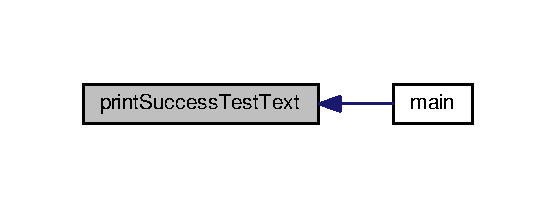
\includegraphics[width=267pt]{test__main_8c_a88f8707e23480970b8ab040b43e6de1f_icgraph}
\end{center}
\end{figure}


\index{test\+\_\+main.\+c@{test\+\_\+main.\+c}!print\+Test\+Text@{print\+Test\+Text}}
\index{print\+Test\+Text@{print\+Test\+Text}!test\+\_\+main.\+c@{test\+\_\+main.\+c}}
\subsubsection[{\texorpdfstring{print\+Test\+Text(char $\ast$test\+Name, char $\ast$text, char $\ast$colour, va\+\_\+list args)}{printTestText(char *testName, char *text, char *colour, va_list args)}}]{\setlength{\rightskip}{0pt plus 5cm}void print\+Test\+Text (
\begin{DoxyParamCaption}
\item[{char $\ast$}]{test\+Name, }
\item[{char $\ast$}]{text, }
\item[{char $\ast$}]{colour, }
\item[{va\+\_\+list}]{args}
\end{DoxyParamCaption}
)}\hypertarget{test__main_8c_a3cce6cf3c9672ca1aa12539a4d0a2ffd}{}\label{test__main_8c_a3cce6cf3c9672ca1aa12539a4d0a2ffd}


Prints a text with a given colour and a list of arguments. 

A wrapper around printf that simplifies printing out test result text in different colours. 
\begin{DoxyParams}{Parameters}
{\em test\+Name} & The name of the test \\
\hline
{\em text} & The text message to print out \\
\hline
{\em colour} & The colour of the text to print \\
\hline
{\em args} & The arguments for the text output, it\textquotesingle{}s a va\+\_\+list so provide it in the same way as for a printf call \\
\hline
\end{DoxyParams}
\begin{DoxyReturn}{Returns}
void 
\end{DoxyReturn}


Here is the caller graph for this function\+:\nopagebreak
\begin{figure}[H]
\begin{center}
\leavevmode
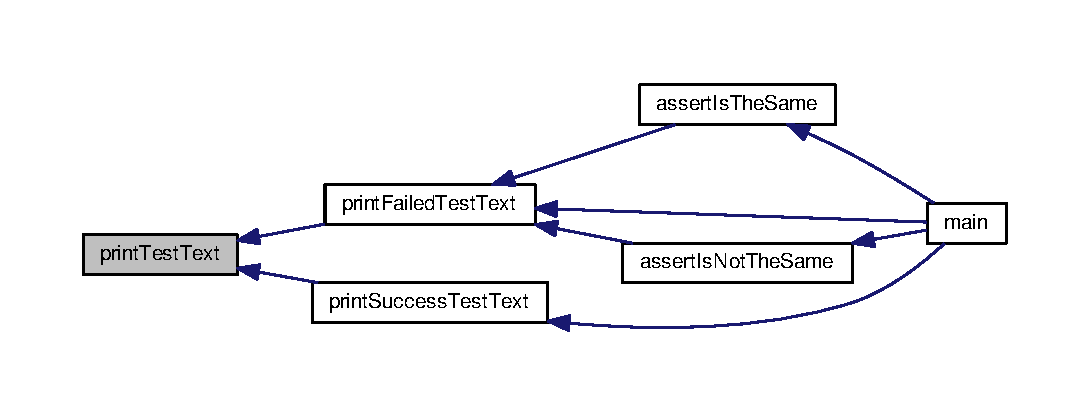
\includegraphics[width=350pt]{test__main_8c_a3cce6cf3c9672ca1aa12539a4d0a2ffd_icgraph}
\end{center}
\end{figure}



%--- End generated contents ---

% Index
\backmatter
\newpage
\phantomsection
\clearemptydoublepage
\addcontentsline{toc}{chapter}{Index}
\printindex

\end{document}
